\documentclass{beamer}

% Theme choice:
\usetheme{CambridgeUS}

% Title page details:
\title{GoTalk}
\author{Swasti \and Shreya \and Krishika \and Samriddhi}
\date{\today}

\begin{document}

% Title frame
\begin{frame}
    \titlepage
\end{frame}

% Idea frame
\begin{frame}{Idea}
    GoTalk will utilize WebSockets for a real-time client-server connection, enabling real-time, bidirectional communication. It will use Firebase for authentication.
\end{frame}

% Aim frame
\begin{frame}{Aim}
    \begin{itemize}
        \item Learn the Go language and Firebase
        \item Learn how to establish a client-server connection using WebSocket and HTTPS
    \end{itemize}
\end{frame}

% Outline frame
\begin{frame}{Outline}
    \tableofcontents
\end{frame}

% Tech Stack section
\section{Tech Stack}
\begin{frame}{Tech Stack}
    \begin{itemize}
        \item \textbf{Frontend}
        \begin{itemize}
            \item HTML/CSS
            \item JavaScript
            \item Bootstrap/Tailwind CSS
        \end{itemize}
        \item \textbf{Backend}
        \begin{itemize}
            \item Go (Golang)
            \item Gorilla WebSocket
            \item HTTP server
            \item Firebase JavaScript SDK
            \item Firebase Realtime Database
        \end{itemize}
    \end{itemize}
\end{frame}

% Timeline section
\section{Timeline}
\begin{frame}{Timeline}
    \begin{block}{Week 1}
        \begin{itemize}
            \item Installation
            \item Basic HTTP server
            \item WebSocket integration
            \item User Authentication using Firebase
        \end{itemize}
    \end{block}
    
    \begin{block}{Week 2}
        \begin{itemize}
            \item Handling messages
            \item Chat history 
            \item User interface
            \item Documentation
        \end{itemize}
    \end{block}
\end{frame}

% Plan of Action section
\section{Plan of Action}
\begin{frame}{Plan of Action}
    \centering
    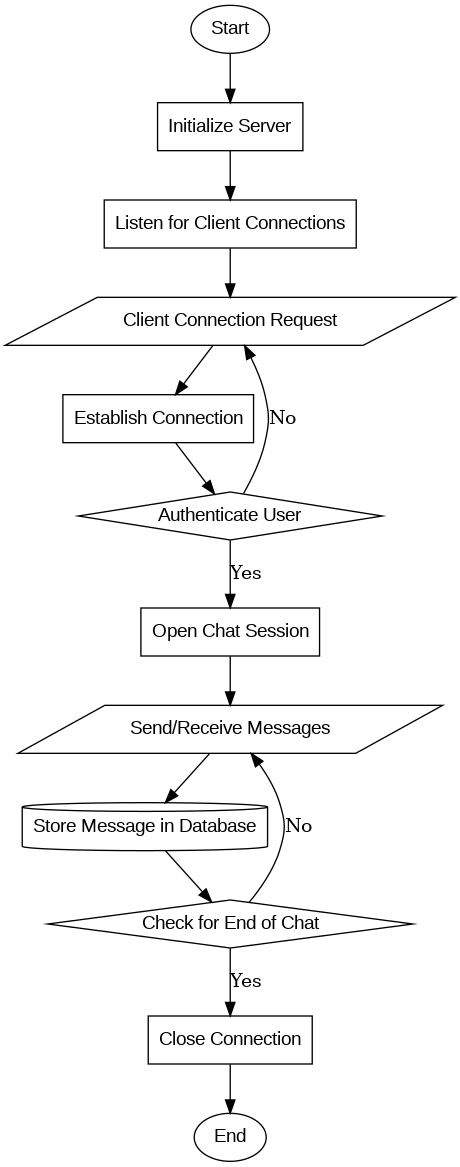
\includegraphics[width=0.25\textwidth]{Graphviz files/Images/graph.png}
\end{frame}

% Procedure frame
\begin{frame}{Procedure}
    \centering
    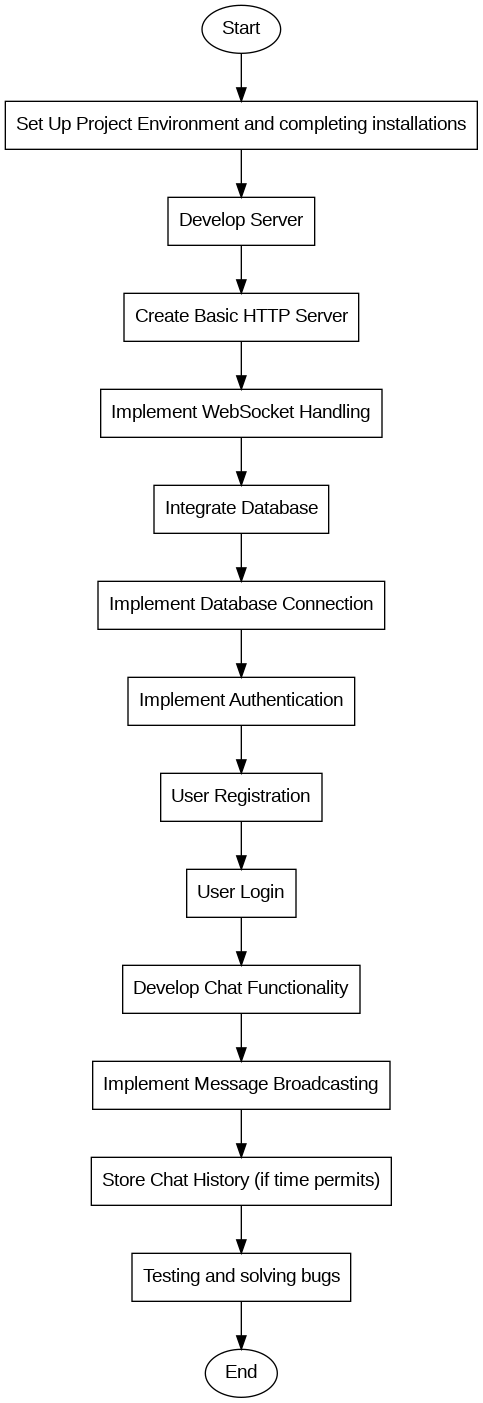
\includegraphics[width=0.22\textwidth]{Graphviz files/Images/implementation.png}
\end{frame}

% Future Scope section
\section{Future Scope}
\begin{frame}{Future Scope}
    \begin{itemize}
        \item Enhanced UI (file attachment, emojis, etc.)
        \item Text Search capabilities
        \item End-to-End Encryption (E2EE)
        \item Polls, community features
    \end{itemize}
\end{frame}

% Thank You frame
\begin{frame}{Thank You}
    \centering
    \Huge Thank You!
\end{frame}

\end{document}
